In this section we introduce the usage of \texttt{ASP} by the use of examples.
The \ASP api is written solely in Python (with the exception of UFL for the weak
form) and thus the user is expected to have a basic knowledge of Python
programming.  However, since \texttt{ASP} is based on the FEniCS/DOLFIN Python
interface it does not compromise on performance\cite{Alnae2011}. The use of
DOLFIN's Python interface allows for greater ease of use, as compared to the C++
interface. Eventually, we intend to offer a GUI which would require the use of
no programming and only entering the details for the domain, boundary
conditions, and the weak form.

\section{Solving a PDE} \label{sec:Solver}

    In this subsection we explain how to solve a basic time dependent PDE using
    the \texttt{ASP} API. We choose to explain the API by example; we choose to
    make things quite simple at first and so the first example is the Heat
    equation.  Since, the FEM requires the weak form of any PDE we assume
    the user understands how to determine the weak form for a given PDE and thus
    no explanation of the weak form is given. For a very basic explanation of
    the weak form see \cite[Chapter 6.2.2]{Eriksson2009}.

    Of course to be able to solve any PDE certain assumptions must be made. \ASP
    makes the assumption that an $H^1$ FE is appropriate for solving the given
    PDE, i.e. the FE discretization is stable. Additionally, \texttt{ASP} assumes the
    PDE has the following form
    \begin{equation}
        R(u) = u_t - F(u;t) = 0,
        \label{eq:BasicForm}
    \end{equation}
    and can be discretized in time in the following way
    \begin{equation}
        r(u^n, u^n, v) = \frac{1}{k} (u^n - u^{n-1}, v) - (F(\hat{u};t^n), v) = 0,
        \label{eq:WeakResidual}
    \end{equation}
    where $u^n,\, u^{n-1},\, \hat{u}$, and $v$ are the solution at the
    $n^{th}$-timestep, the solution at the $(n-1)^{st}$-timestep,
    $\theta$-weighted average of the solution for the $n^{th}$ and
    $(n-1)^{th}$-timestep, i.e.
    \begin{equation}
        \hat{u} = \theta\, u^n + (1 - \theta)\, u^{n-1},
        \label{eq:uAvg}
    \end{equation}
    and the test function, respectively.

    For \ASP, a PDE is defined using the following required objects\slash
    functions \texttt{Problem.T}, \texttt{Problem.t0}, \texttt{Problem.k},
    \texttt{Problem.mesh}, \texttt{Problem.initial\_condition},
    \texttt{Problem.boundary\_conditions}, \texttt{Solver.function\_space}, and
    \texttt{Solver.weak\_residual}, which are the final time (float), initial
    time (float), time-step (float), domain discretization (mesh object),
    initial condition (function), boundary conditions (function), finite element
    space (function), and weak form (function), respectively. The function
    \texttt{Problem.initial\_condition} should return a finite element
    projection of the initial condition, while
    \texttt{Problem.boundary\_conditions} return a list of FEniCS
    \texttt{DirichletBC} objects. Then the function
    \texttt{Solver.function\_space} returns either a \texttt{FunctionSpace}
    object or a \texttt{MixedFunctionSpace} object. The user need not worry too
    much about the definition of these FEniCS objects, but one must know to
    return these types when writing one's functions. These details will become
    much clearer in the following subsection, where we will focus on the
    definition of these objects\slash functions and their use.

    In the example that follows we will demonstrate the use of \ASP through two
    different programming styles: the first method will be by passing function
    handles to the \texttt{Problem} and \texttt{Solver} classes,
    \autoref{sss:FunctionHandles}. This method can be a bit long-winded and thus
    a second method will be demonstrated, which we believe demonstrates the true
    strength of \ASP. This method uses the definition of subclasses to define
    both the \texttt{problem} and the \texttt{solver}, \autoref{sss:Subclasses}.
    With a short script one can easily mix and match problems and solvers. In
    the later sections this method will be the primary method used. In fact, all
    test problems we have written use this script and subclass definition
    method.

\subsection{Heat Equation} \label{sse:Heat}
    The heat equation is a canonical example of parabolic partial differential
    equations. Given the domain $\Omega$ with boundary $\partial \Omega$ and
    time interval $I$ the heat equation is given by
    \begin{equation}
        \begin{split}
            u_t - \nabla \left( \kappa \nabla u \right) &= f
                \qquad (\mathbf{x}, t)\in \Omega \times I \\
            u(\mathbf{x}, 0) &= u_0(\mathbf{x}) \quad \mathbf{x} \in \Omega \\
            u(\mathbf{x}, t) &= g(\mathbf{x},t) \quad (\mathbf{x}, t)\in
                \partial\Omega \times I, \\
        \end{split}
        \label{eq:Heat}
    \end{equation}
    where $f$ is the internal heat source/sink and $g$ is the boundary
    condition. Taking our FE basis functions $v_h\in V^h\subset H^1_0(\Omega)$
    then we are trying to find a $u^n_h \in V^h \subset H^1(\Omega)$ such that
    \begin{equation}
        \frac{1}{k} (u^n - u^{n-1}, v_h) + (\kappa \nabla \hat{u}, \nabla v_h) =
        0 \quad \forall v_h \in V^h,
        \label{eq:WeakHeat}
    \end{equation}
    where $k$ is the time step, $u^n_h$ is the FE solution at the
    $n^{th}$-timestep, $u^{n-1}_h$ is the FE solution at the
    $(n-1)^{st}$-timestep, $\hat{u}$ is given by \eqref{eq:uAvg}, and $\kappa$
    is the heat coefficient. To further
    specify the problem we will define the domain to be the unit square, i.e.
    \begin{equation}
        \Omega := [0, 1] \times [0, 1],
        \label{eq:HeatDomain}
    \end{equation}
    let the initial condition be
    \begin{equation}
        u_0 := \sin(pi\, x)\, \sin(pi\, y)
        \label{eq:HeatIC}
    \end{equation}
    define the function to be
    \begin{equation}
        f(x,y,t) := 0
        \label{eq:HeatSource}
    \end{equation}
    and the boundary condition to be
    \begin{equation}
        g(x,y,t) := 0
        \label{eq:HeatBC}
    \end{equation}

    With the definition of the problem in place we are now ready to move on to
    writing our code. As stated previously, the code for the heat equation will
    be presented in two different fashions, one corresponding to passing
    function handles to class, \autoref{sss:FunctionHandles}, while the other
    consists of created a script and subclasses of \texttt{Problem} and
    \texttt{Solver} classes, \autoref{sss:Subclasses}.

    \subsubsection{Function Handle Method} \label{sss:FunctionHandles}
    Just as in the definition of the PDE \texttt{ASP} requires certain things
    to be defined. First, we can define the mesh (we will use a
    \texttt{UnitSquareMesh} as our domain), and then the mesh must be passed to
    the \texttt{Problem} class. This can be done in the following way
    \lstinputlisting[firstline=63,lastline=68,
        caption={[Unit Square Mesh Creation] Creating a mesh of unit square problem
                domain.}
    ]{Heat.py}
    we need to define the initial conditions and
    boundary conditions. For the initial condition, \eqref{eq:HeatIC}, and
    the boundary condition, \eqref{eq:HeatBC}, these functions can be defined
    as follows
    \lstinputlisting[firstline=10,lastline=20,
        caption={[Heat: ICs and BCs] Create the initial conditions and boundary
        conditions.}
    ]{Heat.py}
    To be able to access these functions \texttt{ASP} needs them define. To do this we
    must pass the functions to \ASP' \texttt{Problem} class. This is done quite
    easily in the following way
    \lstinputlisting[firstline=73,lastline=74,
        caption={[Heat: Passing ICs and BCs] Send initial conditions and
                boundary conditions to \ASP.}
    ]{Heat.py}
    To define the heat source/sink things are actually a bit easier and the user
    need only to pass the function directly to the \texttt{Problem} class. This
    is done in a quite similar way as to the way we passed the ICs and BCs, as
    can be seen below
    \lstinputlisting[firstline=69,lastline=69, label={lst:IC+BC2Problem},
        caption={[Heat: Passing Forcing Fucntion] Send forcing function to
                \ASP.}
    ]{Heat.py}
    In fact, this could be left out if the user does not require it in the weak
    form, but we include it here for completeness.

    Next, we need to create our function space; here we will choose $P^1$ finite
    elements, i.e. piecewise linear basis functions. To do this we create a
    function named \texttt{function\_space}. However, this time we will pass the
    functions to the \texttt{Solver} class. Then we can also define our weak
    form by defining the functions \texttt{weak\_residual}. Similar to
    \texttt{function\_space} we then pass it to the \texttt{Solver} class in the
    same way we passed \texttt{functions\_space}. The definition of the function
    space and the weak form given by \eqref{eq:WeakHeat} can be seen below
    \lstinputlisting[firstline=28,lastline=44,
        caption={[Heat: Function Space and Weak Residual] Defining the function
                space and weak residual}
    ]{Heat.py}
    These functions are then passed to the \texttt{Solver} class in the
    following way
    \lstinputlisting[firstline=80,lastline=81, label={lst:FS+WR2Solver},
        caption={[Heat: Passing Function Space and Weak Residual] Passing our
                function space and weak residual to \texttt{Solver}.}
    ]{Heat.py}

    In addition to the standard functions above, we can define some auxiliary
    functions. Some examples are \texttt{Plot}, \texttt{Name}, and \texttt{Save}
    functions; \texttt{ASP} assumes the equation given is similar to the Navier-Stokes
    equation, i.e. the first variable is a vector function and the second
    variable is a scalar function, thus it may be necessary to override the
    built in functionality so as to fit your own specifics. For this example we
    only override the \texttt{Plot} function; this is done in much the same way
    as we did for the other functions already seen above.
    \lstinputlisting[firstline=47,lastline=54,
        caption={[Heat: Plot] Plot function for post processing.}
    ]{Heat.py}
    \lstinputlisting[firstline=82,lastline=82,
        caption={[Heat: Passing Plot] Passing the plot function to
                \texttt{Solver}}
    ]{Heat.py}

    The entire code can be viewed below
    \lstinputlisting[label={lst:Heat},
        caption={[Heat Equation and Square Problem Code using Function Handle
                Method] Complete code for the Heat equation on a Unit
                Square\eqref{eq:Heat}}
    ]{Heat.py}

    While from a coders point of view this looks more complicated than the
    standard heat equation solver in the FEniCS demos, the beauty of this code
    is that the \texttt{main()} portion of the script remains mostly unchanged
    from problem to problem and from solver to solver. The power of this
    approach can be seen in the code snippets \autoref{lst:FS+WR2Solver} and
    \autoref{lst:IC+BC2Problem}.  With this approach we can easily mix and match
    problems and solvers. Thus, we can use the same main() to run, say, the heat
    equation or even the Navier-Stokes equations (on a simple domain).

    \subsubsection{Subclass Method} \label{sss:Subclasses}

    To demonstrate a very straight forward way to simplify such a script so as
    to use any solver and problem combination we will present the above example
    using subclasses instead of pure function definitions. We will not change
    any of the above functionality, except for placing functions in an
    appropriate subclass. To this end we first present the \texttt{problem}
    which is a subclass of \texttt{ProblemBase}, where \texttt{ProblemBase} is
    the \texttt{Problem} class provided by \ASP.
    \lstinputlisting[firstline=5,
        caption={Square \texttt{Problem} subclass.}
    ]{
        Square.py
    }
    Now we define the \texttt{solver} which will be a subclass of
    \text{SolverBase}, which is the \texttt{Solver} class provided by \ASP.
    \lstinputlisting[firstline=4,
        caption={Heat \texttt{Solver} subclass.}, label={lst:HeatClass}
    ]{
        HeatClass.py
    }

    Finally, one can then solve a particular problem using a script like the
    following.
    \lstinputlisting[caption={[Heat and Square: Solver Script] Solver Script for
        the Heat equation Solver and Square Problem}, label={lst:Script}
    ]{solve.py}

    With the above method one can write a general script to run a variety of
    problem/solver combinations, thus allow for a very easy method to test
    hypothesis without changing much in the way of one's code. This is where the
    main power/attraction lies in using an API such as \ASP. Thus, all code
    which follows will be presented in this form and the script use to run the
    various problem will be assumed to be quite similar to the script presented
    in \autoref{lst:Script}.

\section{Goal Oriented Adaptivity} \label{sec:Adaptivity}

    In this subsection we will introduce Goal Oriented Adaptivity as used in
    \ASP.  The details for the goal oriented adaptivity algorithm used by \ASP
    can be seen in \cite{Foster2014e,Jansson2014a,Jansson2014b}. Again we will
    demonstrate this functionality by example. The following subsections will
    present two examples: the first example will present the
    Advection-Reaction-Diffision equation solved on a domain with a hole, the
    next example is flow around a cylinder using the Navier-Stokes equation.
    This last example will demonstrate how to solve a non-linear PDE, the use of
    mixed finite element spaces, and how to use goal oriented adaptivity.  The
    addition of goal oriented adaptivity is quite simple and the only required
    intervention by the user is the creation of a goal functional,
    \texttt{Problem.functional}, and the setting of the boolean
    \texttt{options['adaptivity']} to true.  Additionally, the user should
    notice th  \texttt{ei\_mode} boolean is passed to
    \texttt{Solver.weak\_residual}, so that the user can change behavior while
    calculating the error indicators.

    \begin{remark}
        We must mention that the stabilization for our formulation will be
        turned off during the calculation of error indications, i.e. during
        \texttt{ei\_mode}. Thus, the function \texttt{weak\_residual} is
        presented again, only for completeness.
    \end{remark}

\subsection{Advection-Reaction-Diffusion Equation} \label{sse:ADR}
    In this subsection we extend what was done for the Heat Equation,
    \autoref{sse:Heat}, to that of the Advection-Reaction-Diffusion equation
    (ADR). The ADR is a simple linear model of a reactive and diffusive flow. In
    what follows the parameters $\alpha,\,\beta$, and $\kappa$ represent the
    reactivity, convective velocity vector, and diffusivity tensor,
    respectively. Thus, for $t\in [0,T]$ and a domain $\Omega$ with boundary
    $\partial \Omega$, the ADR is given by
    \begin{equation}
        \begin{split}
            u_t + \nabla \left(\kappa\cdot \nabla u \right) + \beta \cdot \nabla
                u + \alpha u = f,& \quad \mathbf{x} \in \omega, \\
            u = g,& \quad \mathbf{x} \in \partial \omega, \\
            u = 0,& \quad t = 0,\, \mathbf{x} \in \partial \omega,
        \end{split}
        \label{eq:ADR}
    \end{equation}
    where $f$ is the external forcing.

    For this particular example we take the domain to be a square domain with a
    center square removed. That is we take the outer square to be $\Omega_1$ and
    the inner square to be $\Omega_2$ and the resulting domain $\Omega$ is given
    by
    \begin{equation}
        \Omega = \Omega_1\setminus \Omega_2,
        \label{eq:ADRDomain}
    \end{equation}
    and then the boundary $\partial \Omega$ is defined as
    \begin{equation}
        \partial \Omega = \partial \Omega_1 + \partial \Omega_2,
        \label{eq:ADRBoundary}
    \end{equation}
    where $\partial \Omega_1$ is the boundary of $\Omega_1$ and $\partial
    \Omega_2$ is the boundary of $\Omega_2$ (see \autoref{fig:ADRDomain}.

    \begin{figure}[h]
        \centering
        \tikzstyle{next}=[->, thick, shorten <=1pt, shorten >=1pt]
        \begin{tikzpicture}[scale=6]
            \draw (0,0) -- (1,0) -- (1,1) -- (0,1) -- cycle;
            \draw (0.4,0.4) -- (0.6,0.4) -- (0.6,0.6) -- (0.4,0.6) -- cycle;
            \node (Omega_2) at (0.5,0.5) {$\Omega_2$};
            \node (dOmega_2) at (0.5,0.65) {$\partial\Omega_2$};
            \node (Omega_1) at (0.25,0.25) {$\Omega_1$};
            \node (dOmega_1) at (0.5,0.05) {$\partial\Omega_1$};
        \end{tikzpicture}
        \caption{Problem Geometry, $\Omega$, for ADR small hole problem.}
        \label{fig:ADRDomain}
    \end{figure}

    Furthermore, in this example we will take the subdomains to be $\Omega_1 =
    [0,1]^2$ and $\Omega_2 = [0.48,0.52]^2$. With these subdomains defined we
    take the boundary condition to be
    \begin{equation}
        g = \begin{cases}
            0   &\mathbf{x} \in \partial \Omega_1 \\
            5 + 5\, \sin \pi\, t  &\mathbf{x} \in \partial \Omega_2
        \end{cases}.
        \label{eq:ADRBCs}
    \end{equation}
    Finally we take the final time $T=10,\, \alpha=1,\, \beta = \left[ -1,
    -0.61 \right]$, and $\kappa = 1\times10^{-5}$.

    We will discretize ADR using a Galerkin\slash Least-Squares (GLS) stabilized
    cG(1)cG(1) finite element, where the first cG(1) indicates that the test and
    trial functions are both piecewise linear, while the second cG(1) indicates
    that the test piecewise constants and the trial functions are continuous
    piecewise linear (see \cite{Hoffman2006a} for more details).

    Given a step size $k$ and applying the cG(1)cG(1) finite element
    discretization to \eqref{eq:ADR} with $v \in X \subset H^1_0(\Omega)$ gives
    the following weak residual
    \begin{equation}
    \begin{split}
        r(\bar{u}^n; v) &= \left(u^n - u^{n-1}\right)\,k^{-1}
            + (\kappa \nabla \bar{u}^n, \nabla v)
            + (\beta \cdot \nabla \bar{u}^n, v) + (\alpha u, v) - (f, v) = 0
    \end{split}
    \label{eqn:WeakADR}
    \end{equation}
    where $\bar{u}^n = \frac{1}{2}\left(u^n + u^{n-1}\right)$. Given the
    solution $u$, since the elements we are concerned with (cG(1)cG(1)) have
    test functions which are linear in space and constant in time the strong
    residual is given by
    \begin{equation}
        R(u) = \alpha u + \beta \cdot \nabla u - f
    \label{eqn:StrongADR}
    \end{equation}
    Finally, the GLS stabilized cG(1)cG(1) discretization of \eqref{eq:ADR} is
    given by
    \begin{equation}
        r(\bar{u}^n,v) + SD_{\delta}^n(\bar{u}^n,v) = 0,
            \quad \forall v \in X.
        \label{eqn:G2ADR}
    \end{equation}
    Here $SD_{\delta}^n$ is the GLS stabilization and is given by
    \begin{equation}
        SD_{\delta}^n(\bar{u}^n, v) \equiv \delta \left(R(\bar{u}^n), R(v)
            + f\right)
    \label{eq:ADRStabilization}
    \end{equation}
    where
    \begin{equation}
        \delta = \begin{cases}
            \frac{h^2}{\|\beta\|} & \text{if } h \le \kappa \\
            \frac{h}{\|\beta\|} & \text{otherwise}
        \end{cases}
        \label{eq:ADRdelta}
    \end{equation}
    Additionally, we take the time-step to be
    \begin{equation*}
        k = CFL\, \min_{\mathcal{T}_K}(h),
    \end{equation*}
    where $CFL=100$.

    \lstinputlisting[firstline=5,
        caption={ADR Domain \texttt{Problem} subclass.}, label={lst:ADRDomain}
    ]{SmallHole.py}
    \lstinputlisting[firstline=5,
        caption={ADR \texttt{Solver} subclass.}, label={lst:ADR}
    ]{ADR.py}
    \begin{figure}[h]
        \centering
        \begin{minipage}[t]{0.49\textwidth}
            \centering
            \subcaptionbox{Starting mesh.}{
                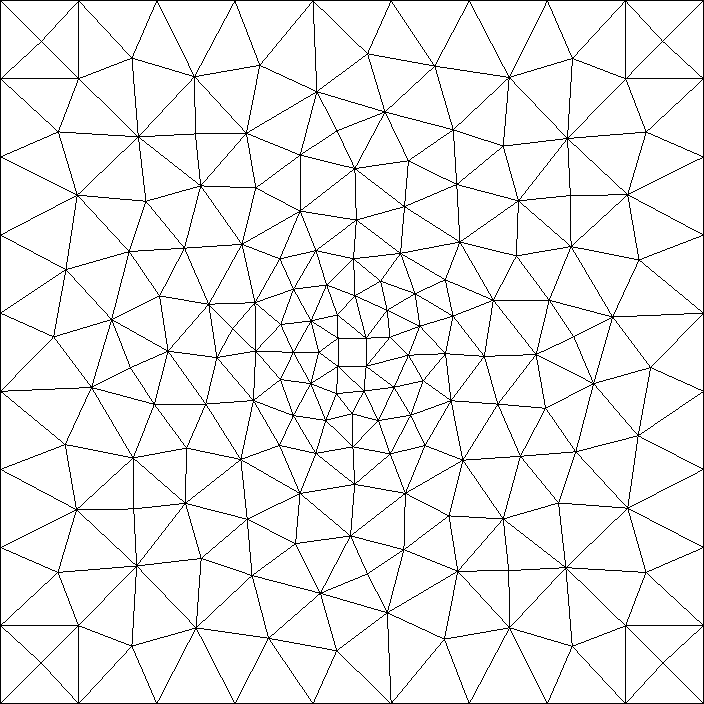
\includegraphics[scale=0.16]{Figures/AdaptiveADRkappa1E-5_mesh0.png}
            }
            \subcaptionbox{Primal solution from starting mesh.}{
                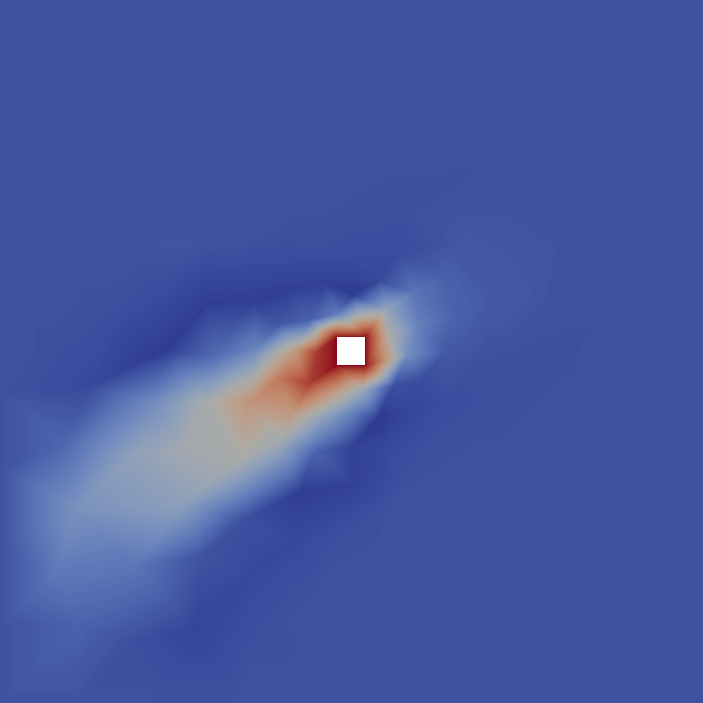
\includegraphics[scale=0.16]{Figures/AdaptiveADRkappa1E-5_u0.png}
            }
            \subcaptionbox{Error indicators from starting mesh.}{
                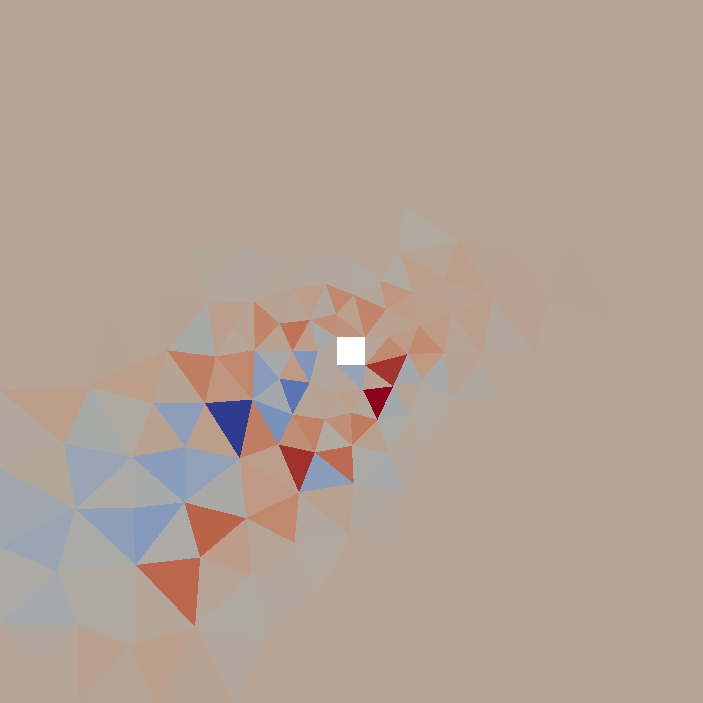
\includegraphics[scale=0.16]{Figures/AdaptiveADRkappa1E-5_ei0.png}
            }
            \subcaptionbox{Dual solution from starting mesh.}{
                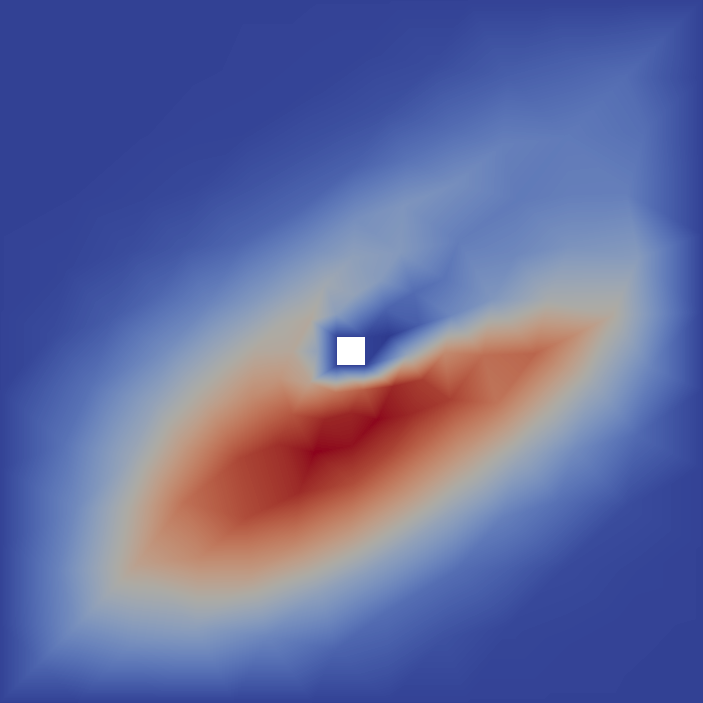
\includegraphics[scale=0.16]{Figures/AdaptiveADRkappa1E-5_uDual0.png}
            }
        \end{minipage}
        \begin{minipage}[t]{0.49\textwidth}
            \centering
            \subcaptionbox{$27^{th}$ adaptive mesh.}{
                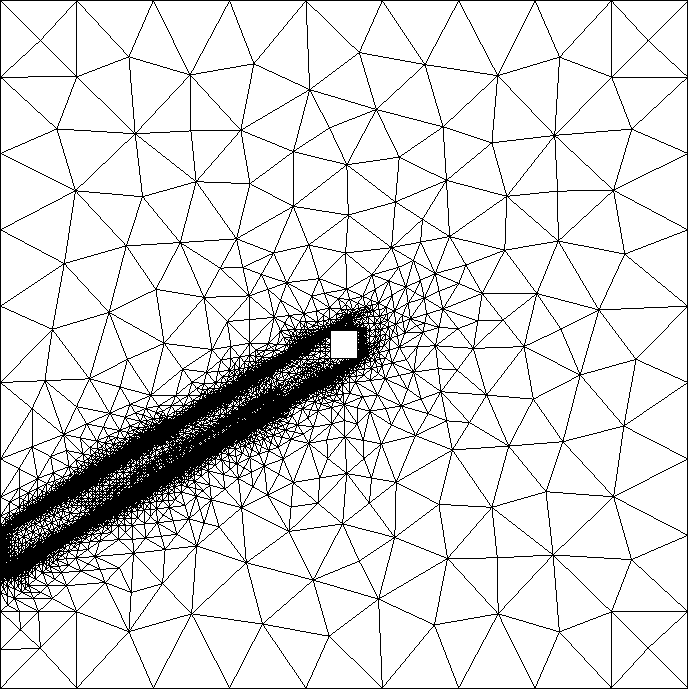
\includegraphics[scale=0.162]{Figures/AdaptiveADRkappa1E-5_mesh27.png}
            }
            \subcaptionbox{Primal solution after 27 adaptive iterations.}{
                
\includegraphics[scale=0.162]{Figures/AdaptiveADRkappa1E-5_u27.png}
            }
            \subcaptionbox{Error indicators after 27 adaptive iterations.}{
                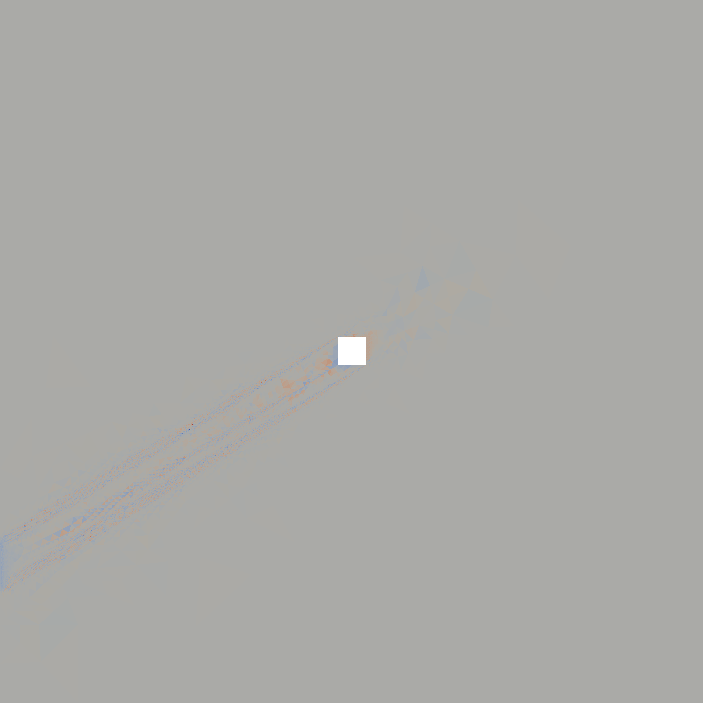
\includegraphics[scale=0.162]{Figures/AdaptiveADRkappa1E-5_ei27.png}
            }
            \subcaptionbox{Dual solution after 27 adaptive iterations.}{
                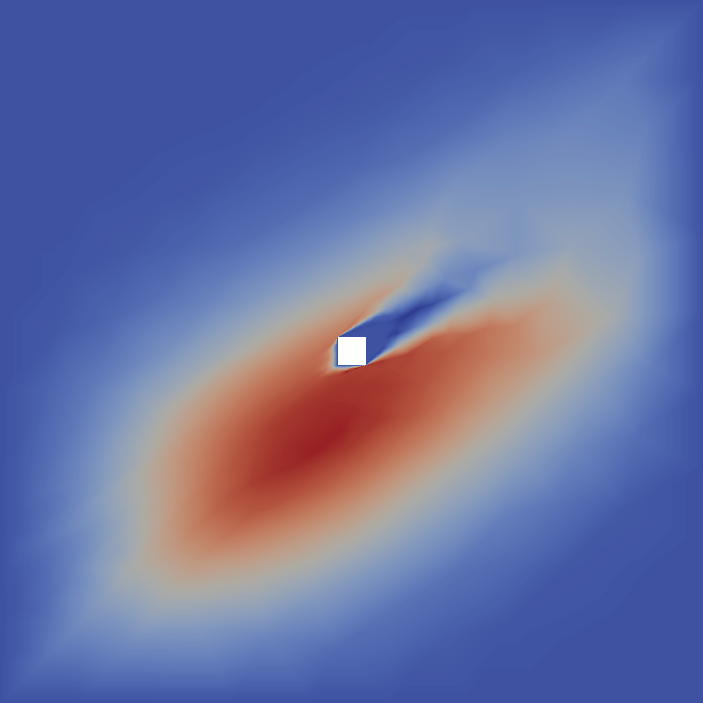
\includegraphics[scale=0.162]{Figures/AdaptiveADRkappa1E-5_uDual27.png}
            }
        \end{minipage}
        \caption{Results for ADR Small Hole problem with
            $\kappa=1\times10^{-5}$.}
    \end{figure}

    \begin{figure}[h]
        \centering
        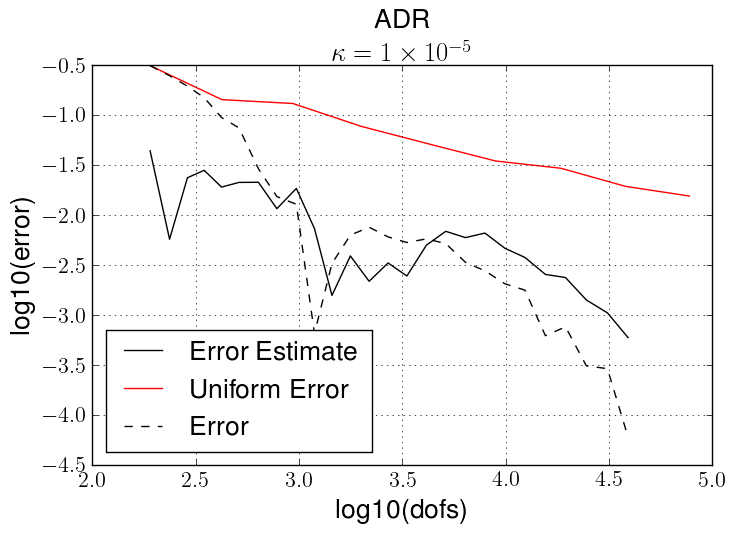
\includegraphics[scale=0.5]{Figures/AdaptiveADRkappa1E-5.png}
        \caption{Adaptive error estimate versus ``true'' error for the solution
            for the ADR equation.}
        \label{fig:ADR_err}
    \end{figure}

\subsection{Navier-Stokes Equations} \label{sse:NSE}

    In this subsection we demonstrate the use of \texttt{ASP} on a more complicated
    example, one that includes a non-linear term, namely the Navier-Stokes
    equations for flow around a cylinder.  Again, we will discretize the
    Navier-Stokes equations using a GLS stabilized cG(1)cG(1) finite element.

    For this problem we are concerned with modelling the incompressible
    Navier-Stokes equations (NSE) with constant kinematic viscosity, $\nu>0$, in
    a domain $\Omega\subset \R^d$, with boundary $\partial \Omega$, i.e.  where
    the strong residual is given by
    \begin{equation}
        \begin{split}
            \mathbf{u}_t + \left( \mathbf{u} \cdot \nabla \right) \mathbf{u}
                - \nu\, \Delta \mathbf{u} + \nabla p = \mathbf{f},
                    \quad \mathbf{x} \in \Omega \\
            \nabla \cdot \mathbf{u} = 0, \quad \mathbf{x} \in \Omega
        \end{split}
    \label{eqn:NSE}
    \end{equation}
    Given a step size $k$ and applying the cG(1)cG(1) finite element discretization
    to \eqref{eqn:NSE} with $V = (v, q) \in X \subset [H^1_0(\Omega)]^d \times
    H^1(\Omega)$ gives the following weak residual
    \begin{equation}
    \begin{split}
        r(\bar{U}^n; V) &= \left(\mathbf{u}^n - \mathbf{u}^{n-1}\right)\,k^{-1}
            + (\left( \bar{\mathbf{u}}^n \cdot \nabla \right) \bar{\mathbf{u}}^n, v) \\
            &\quad+ \nu\, (\nabla \bar{\mathbf{u}}^n, \nabla v)
            + (\nabla p^n, v) - (\mathbf{f}, v)
            + (\nabla \cdot \bar{\mathbf{u}}^n, v) = 0
    \end{split}
    \label{eqn:WeakNSE}
    \end{equation}
    where $U^n = (\mathbf{u}, p)$ and $\bar{U}^n = \frac{1}{2}\left(U^n +
    U^{n-1}\right)$. Given the solution $U$, since the elements we are concerned
    with (cG(1)cG(1)) have test functions which are linear in space and constant
    in time the strong residual is given by
    \begin{equation}
        R(U,V) = \begin{cases}
                \left(\mathbf{v} \cdot \nabla \right) \mathbf{u}
                + \nabla \bar{p}^n - \mathbf{f} = 0 \\
            \nabla \cdot \mathbf{u} = 0.
        \end{cases}
    \label{eqn:StrongNSE}
    \end{equation}
    Finally, the GLS stabilized cG(1)cG(1) discretization of \eqref{eqn:NSE} is
    given by
    \begin{equation}
    r(\bar{U}^n,V) + SD_{\delta}^n(\bar{U}^n,V) = 0, \quad \forall V = (v,q) \in X.
    \label{eqn:G2}
    \end{equation}
    Here $SD_{\delta}^n$ is the GLS stabilization and is given by
    \begin{equation}
        SD_{\delta}^n(\bar{U}^n, V) \equiv
        \delta \left[(\left(\bar{\mathbf{u}}^n \cdot \nabla \right) \bar{\mathbf{u}}^n
            + \nabla p^n - \mathbf{f},
        \left(\bar{\mathbf{u}}^n \cdot \nabla \right) v + \nabla q)
            + (\nabla \cdot \bar{\mathbf{U}}^n, \nabla \cdot v)\right],
    \label{eqn:NSEStabilization}
    \end{equation}
    where
    \begin{equation*}
        \delta = \begin{cases}
            h^2 & \text{if } h < \nu \\
            h & \text{otherwise}
        \end{cases}
    \end{equation*}
    For each test case below we take the time-step to be
    \begin{equation*}
    k = CFL\, \frac{\min_{\mathcal{T}_K}(h)}{|U_m|},
    \end{equation*}
    where $CFL=100$.

    This test case is based on a benchmark problem from Sch\"afer and Turek
    \cite[Test case 2D-2]{Schaefer1996}. Thus, we define the domain to be a
    rectangular domain with a circle removed (see \autoref{fig:2DCylinder}). For
    the inlet boundary condition we take
    \begin{equation}
        u(0,y,t) = (4\, U_m\,y\, (H - y)/H^2, 0),
        \label{eqn:2DInlet}
    \end{equation}
    where $U_m = 1.5\, \text{m/s}$, $H = 0.41\, \text{m}$. For the kinematic
    viscosity we take $\nu = 10^{-3}\, \text{m}^2\text{/s}$, resulting in a
    Reynolds number of $Re=100$.

    \begin{figure}[h]
        \centering
        \tikzstyle{next}=[->, thick, shorten <=1pt, shorten >=1pt]
        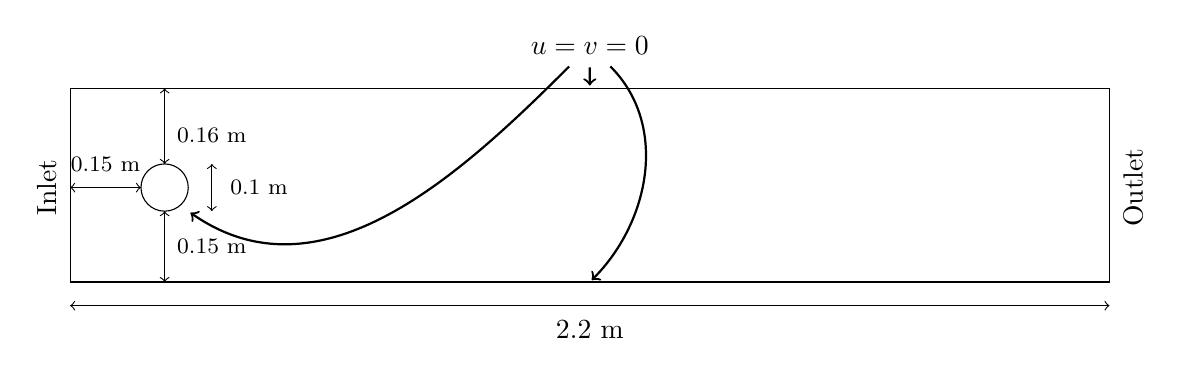
\begin{tikzpicture}[scale=6]
            \draw (0,0) -- (2.2,0) -- (2.2,0.41) -- (0,0.41) -- cycle;
            \draw (0.2,0.2) circle (0.05);
            \draw[<->] (0,-0.05) -- (2.2,-0.05);
            \draw (1.1,-0.1) node {2.2 m};
            \draw[<->] (0,0.2) -- (0.15,0.2);
            \draw (0.075,0.25) node {\footnotesize 0.15 m};
            \draw[<->] (0.2,0) -- (0.2,0.15);
            \draw (0.3,0.075) node {\footnotesize 0.15 m};
            \draw[<->] (0.2,0.25) -- (0.2,0.41);
            \draw (0.3,0.31) node {\footnotesize 0.16 m};
            \draw[<->] (0.3,0.15) -- (0.3,0.25);
            \draw (0.4,0.2) node {\footnotesize 0.1 m};
            \node[rotate=90] (outflow) at (2.25, 0.2) {Outlet};
            \node[rotate=90] (inflow) at (-0.05, 0.2) {Inlet};
            \node (NoFlow) at (1.1,0.5) {$u=v=0$};
            \draw[next] (NoFlow) to (1.1,0.41);
            \draw[next] (NoFlow) to [out=-45,in=45] (1.1,0);
            \draw[next] (NoFlow) to [out=-135,in=-35] (0.25,0.15);
        \end{tikzpicture}
        \caption{Problem Geometry for NSE flow around a cylinder, $\Omega$}
        \label{fig:2DCylinder}
    \end{figure}

    Finally, we choose a simple goal functional, namely the average velocity in
    the $x$-direction, i.e.
    \begin{equation}
        \int_{I}\!\int_{\Omega} u\, d\mathbf{x}\,dt.
        \label{eq:NSEGoal}
    \end{equation}

    For much of this example the code is quite similar to the previous example,
    \autoref{lst:Heat}.  Some differences come from the more complex geometry,
    time dependent boundary conditions, and stabilization. One additional
    complexity is the non-linearity inherent to the Navier-Stokes equations
    which does not exist in the Heat equation. \texttt{ASP} assumes all problems
    are non-linear, and therefore no changes must be made to take into account a
    non-linear problem.  It should, however, be mentioned that this assumption
    by \texttt{ASP} does tend to slow the calculations down for linear problem.
    As for the other complexity added by flow around a cylinder, \texttt{ASP}
    handles the additionally complexity in a straight forward manner that is
    similar to what one would expect in the standard Python interface of
    FEniCS/DOLFIN.

    The first step we take is setting up problem specific parameters, including
    definition of geometric extent, maximum velocity, etc.
    \lstinputlisting[firstline=6,lastline=16,
        caption={Importing \texttt{ASP} and problem specific parameter
                 definitions for flow around a cylinder.}
    ]{Cylinder.py}
    \lstinputlisting[firstline=58, lastline=93, caption={Initialization of
        problem, which includes settings parameters and mesh creation.}
    ]{Cylinder.py}
    Then in the same way we did in the previous example we setup the initial
    conditions and send them to \texttt{Problem}
    \lstinputlisting[firstline=19,lastline=26, label={lst:ICExpNSE},
        caption={Expression for the initial conditions for Navier-Stokes
                equations}
    ]{Cylinder.py}
    \lstinputlisting[firstline=95,lastline=100, label={lst:ICNSE},
        caption={Initial conditions for Navier-Stokes equations}
    ]{Cylinder.py}

    Next we define the various boundaries, which include the inflow, outflow,
    and no-slip boundaries (the cylinder is considered a no-slip boundary), then
    we define the boundary conditions
    \lstinputlisting[firstline=28,lastline=48, label={lst:SubDomainsNSE},
        caption={Defining problem specific boundaries for flow around a
            cylinder.}
    ]{Cylinder.py}
    \lstinputlisting[firstline=106,lastline=120, label={lst:BCsNSE},
        caption={Defining boundary conditions for Cylinder problem}
    ]{Cylinder.py}

    Since our boundary conditions are not constant we must allow for the
    boundary conditions to be updated. To do this we add the update function to
    \texttt{Problem}, which is done in much the same way as the other functions
    we have added up until now
    \lstinputlisting[firstline=130, lastline=132, caption={Update boundary
        conditions for the Cylinder problem.}
    ]{Cylinder.py}

    \begin{remark}
        We note that the update function is called at the beginning
        of each time step.
    \end{remark}

    We must also define the forcing functions, which is simply done by defining
    functions with the names corresponding to the names used in the solver
    definition (used later), i.e.
    \lstinputlisting[firstline=122,lastline=128, caption={Forcing functions for
        the Cylinder problem}
    ]{Cylinder.py}

    Next we define the goal functional, \eqref{eq:NSEGoal}, to be used for goal
    oriented adaptivity.
    \lstinputlisting[firstline=134,lastline=141, label={lst:Functional},
        caption={Goal functional for the Cylinder problem.}
    ]{Cylinder.py}

    Now that the problem has been defined we then proceed by defining the
    solver. Again, the steps here are quite similar to how we did things in the
    Heat equation, except that we do things by a subclass.  To do this we define
    a \texttt{Solver} subclass which must contain, at least, the function
    \texttt{weak\_residual} and the function \texttt{function\_space}. For our
    implementation of NSE we must include stabilization terms, here we choose to
    do so by defining a function \texttt{strong\_residual}.  This can be seen in
    the following lines, since things are done through a \texttt{Solver}
    subclass passing of the functions \texttt{function\_space},
    \texttt{weak\_residual}, and \texttt{strong\_residual} to the
    \texttt{Solver} class is no longer needed.

    First, we define initialize the \texttt{Solver} subclass
    \lstinputlisting[firstline=5,lastline=17,
        caption={Importing \texttt{ASP} and initializing the NSE
                 \texttt{Solver} subclass}
    ]{NSE.py}

    Next, we will define our \texttt{function\_space},
    \texttt{strong\_residual}, and \texttt{weak\_residual} functions.
    \lstinputlisting[firstline=19,lastline=65,
        caption={Defining the \texttt{function\_space},
                 \texttt{strong\_residual}, and \texttt{weak\_residual}.}
    ]{NSE.py}

    Now, to set \texttt{ASP} to use adaptivity we must set the option for
    adaptivity to true. This is easily done before initializing the
    \texttt{Solver} in one's script using the following code
    \begin{lstlisting}[label={lst:AdaptiveBool},
                       caption={Setting the the adaptive boolean to true.}]
        options['adaptive'] = True
    \end{lstlisting}

    The addition of the functional, \autoref{lst:Functional}, and setting the
    adaptive option to true, \autoref{lst:AdaptiveBool}, are the only necessary
    additions needed for goal oriented adaptivity in the Navier-Stokes equation.
    Most applications of the goal oriented adaptivity will be quite similar and
    won't need any real changes.

    Below are the complete codes for the definition of the \texttt{Problem}
    subclass and the \texttt{Sovler} subclass.
    \lstinputlisting[firstline=6,label={lst:NSEClass},
        caption={Cylinder \texttt{Problem} subclass.}
    ]{Cylinder.py}

    \lstinputlisting[firstline=5,label={lst:CylinderClass},
        caption={NSE \texttt{Solver} subclass.}
    ]{NSE.py}

    \begin{figure}[h]
        \centering
        \begin{minipage}[t]{0.49\textwidth}
            \centering
            \subcaptionbox{Starting mesh.}{
                \includegraphics[scale=0.16]{Figures/AdaptiveCylinderRe100_mesh0.png}
            }
            \subcaptionbox{Primal solution from starting mesh.}{
                \includegraphics[scale=0.16]{Figures/AdaptiveCylinderRe100_u0.png}
            }
            \subcaptionbox{Error indicators from starting mesh.}{
                \includegraphics[scale=0.16]{Figures/AdaptiveCylinderRe100_ei0.png}
            }
            \subcaptionbox{Dual solution from starting mesh.}{
                \includegraphics[scale=0.16]{Figures/AdaptiveCylinder100_uDual0.png}
            }
        \end{minipage}
        \begin{minipage}[t]{0.49\textwidth}
            \centering
            \subcaptionbox{$27^{th}$ adaptive mesh.}{
                \includegraphics[scale=0.162]{Figures/AdaptiveCylinderRe100_mesh27.png}
            }
            \subcaptionbox{Primal solution after 27 adaptive iterations.}{
                \includegraphics[scale=0.162]{Figures/AdaptiveCylinderRe100_u27.png}
            }
            \subcaptionbox{Error indicators after 27 adaptive iterations.}{
                \includegraphics[scale=0.162]{Figures/AdaptiveCylinderRe100_ei27.png}
            }
            \subcaptionbox{Dual solution after 27 adaptive iterations.}{
                \includegraphics[scale=0.162]{Figures/AdaptiveCylinderRe100_uDual27.png}
            }
        \end{minipage}
        \caption{Results for NSE flow around a cylinder $Re=100$.}
    \end{figure}
    \begin{figure}[h]
        \centering
        \includegraphics[scale=0.5]{Figures/AdaptiveCylinderRe100.png}
        \caption{Adaptive error estimate versus ``true'' error for the solution
            of the NSE.}
        \label{fig:NSE_err}
    \end{figure}

%\section{Optimization} \label{sec:Optimization}
